\paragraph{QuizziPedia::Front-End::ModelViews::MenuBarModelView}

\label{QuizziPedia::Front-End::ModelViews::MenuBarModelView}

\begin{figure}[ht]
	\centering
	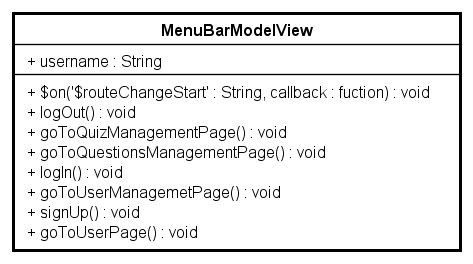
\includegraphics[scale=0.5,keepaspectratio]{UML/Classi/Front-End/QuizziPedia_Front-end_ModelView_MenuBarModelView.png}
	\caption{QuizziPedia::Front-End::ModelViews::MenuBarModelView}
\end{figure} \FloatBarrier

\begin{itemize}
	\item \textbf{Descrizione}: classe di tipo modelview la cui istanziazione è contenuta all'interno della variabile di ambiente \$scope di \textit{Angular.js\ped{G}}. All'interno di essa sono presenti le variabili e i metodi necessari per il \textit{Two-Way Data-Binding\ped{G}} tra la view \texttt{Index} e il controller \texttt{MenuBarController};
	\item \textbf{Utilizzo}: viene utilizzata per effettuare il \textit{Two-Way Data-Binding\ped{G}} tra la view \texttt{Index} e il controller \texttt{MenuBarController} rendendo disponibili variabili e metodi;
	\item \textbf{Relazioni con altre classi}: 
	\begin{itemize}
		\item \textit{OUT} \texttt{LoginBarDirective}: directive contenente il componente che permette di effettuare il redirect alla pagina di login;
		\item \textit{OUT} \texttt{SignUpBarDirective}: directive contenente il componente che permette di effettuare il redirect alla pagina di registrazione;
		\item \textit{OUT} \texttt{UserBarDirective}: directive contenente il componente che permette di effettuare il redirect alla pagina di visualizzazione del profilo utente personale;
		\item \textit{OUT} \texttt{ProfileManagementBarDirective}: directive contenente il componente che permette di effettuare il redirect alla pagina di gestione del profilo;
		\item \textit{OUT} \texttt{QuestionsManagementBarDirective}: directive contenente il componente che permette di effettuare il redirect alla pagina di gestione delle domande;
		\item \textit{OUT} \texttt{LogoutBarDirective}: directive contenente il componente che permette di effettuare il logout;
		\item \textit{OUT} \texttt{QuestionnaireManagementBarDirective}: directive contenente il componente che permette di effettuare il redirect alla pagina di gestione dei questionari;
		\item \textit{OUT} \texttt{MenuBarController}: questa classe permette di gestire il menù fisso per ogni pagina.
	\end{itemize}
	\item \textbf{Attributi}: 
	\begin{itemize}
		\item \texttt{+ username: String} \\ Attributo che conterrà l'username dell'utente.
	\end{itemize}
	\item \textbf{Metodi}: 
	\begin{itemize}
		\item \texttt{+} \texttt{logOut(): void} \\
		Metodo che richiama il metodo \texttt{logOut} del service \texttt{AuthService} passandogli lo \texttt{username}. Prima di effettuare questa operazione viene mostrato a video un messaggio di conferma per il proseguo dell'operazione; 
		\item \texttt{+} \texttt{logIn(): void} \\
		Metodo che gestisce l’evento click sul pulsante per effettuare il login. Effettua il redirect alla pagina per effettuare il login; 
		\item \texttt{+} \texttt{signUp(): void} \\
		Metodo che gestisce l’evento click sul pulsante per effettuare la registrazione. Effettua il redirect alla pagina per effettuare la registrazione; 
		\item \texttt{+} \texttt{goToUserPage(): void} \\
		Metodo che gestisce l’evento click sul pulsante di visualizzazione della pagina utente. Effettua il redirect alla pagina di visualizzazione della pagina utente; 
		\item \texttt{+} \texttt{goToUserManagemetPage(): void} \\
		Metodo che gestisce l’evento click sul pulsante di gestione del profilo utente. Effettua il redirect alla pagina di gestione del profilo utente; 
		\item \texttt{+} \texttt{goToQuestionsManagementPage(): void} \\
		Metodo che gestisce l’evento click sul pulsante di gestione delle domande. Effettua il redirect alla pagina di gestione delle domande; 
		\item \texttt{+} \texttt{goToQuizManagementPage(): void} \\
		Metodo che gestisce l’evento click sul pulsante di gestione dei questionari. Effettua il redirect alla pagina di gestione dei questionari;
		\item \texttt{+ \$on('\$routeChangeStart': String, callback: function): void} \\
		Metodo che cattura i cambiamenti dell'url e che richiede al \texttt{MenuBarModel} le giuste direttive da inserire in \texttt{MenuBarDirective}. \\
		\textbf{Parametri};
		\begin{itemize}
			\item \texttt{'\$routeChangeStart': String}	\\ Servizio offerto da \textit{Angular.js\ped{G}} per catturare gli eventi sulla barra degli URL;
			\item \texttt{callback: function}	\\ Funzione di callback per gestire i cambiamenti della barra degli indirizzi.
		\end{itemize}
	\end{itemize}
\end{itemize}

